\subsection{RISC-V ISA}
\label{subsection:ISA}
The instructions have a 3-operand format: a target register \textit{Rd} and two source registers \textit{Rs1} and \textit{Rs2}. Instructions are divided into different types according to format:\\

\begin{description}
	\item \textbf{R-type:}
  \begin{figure}[h]
    \center
    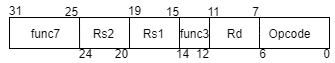
\includegraphics[width=0.7\textwidth]{sec1/images/Rtype.png}
  \end{figure}
	\begin{description}
		\item Operands:\\
		\texttt{Rd, Rs1, Rs2}
		\item Instructions:\\
		\textsf{ADD x2, x4, x6}\ \ \ \ $\longrightarrow$ \ \ \ \ \texttt{x2 = x4 + x6} \\
    \textsf{XOR x2, x4, x6}\ \ \ \ $\longrightarrow$ \ \ \ \ \texttt{x2 = x4 $\oplus$ x6} \\
    \textsf{SLT x2, x4, x6}\ \ \ \ $\longrightarrow$ \ \ \ \ \texttt{ if x4 < x6, x2 = 1 else x2 = 0}
	\end{description}
	\item \textbf{I-type:}
  \begin{figure}[h]
    \center
    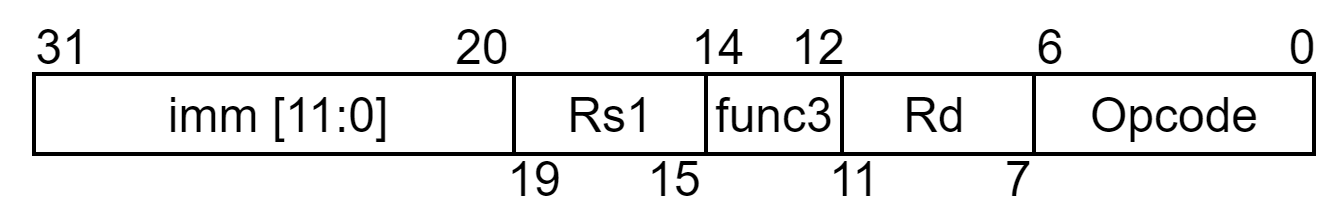
\includegraphics[width=0.7\textwidth]{sec1/images/Itype.png}
  \end{figure}
	\begin{description}
		\item Operands:\\
		\texttt{Rd, Rs1, Immed-12}
		\item Instructions:\\
		\textsf{ADDI x2, x4, 20}\ \ \ \ $\longrightarrow$ \ \ \ \ \texttt{x2 = x4 + 20} \\
		\textsf{LW x7, 8(x4)}\ \ \ \ $\longrightarrow$ \ \ \ \ \texttt{x7 = MEM[x4 + 8]} \\
    \textsf{ANDI x2, x4, 20}\ \ \ \ $\longrightarrow$ \ \ \ \ \texttt{x2 = x4 $\cdot$ 20}
	\end{description}
	\item \textbf{S-type:}
  \begin{figure}[h]
    \center
    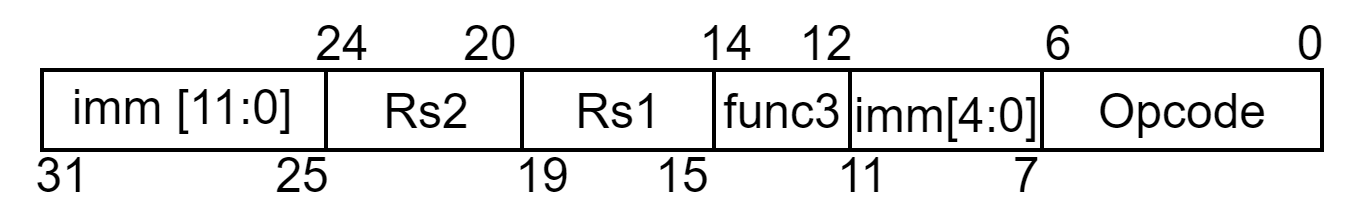
\includegraphics[width=0.7\textwidth]{sec1/images/Stype.png}
  \end{figure}
	\begin{description}
		\item Operands:\\
		\texttt{Rs1, Rs2, Immed-12}
		\item Instruction:\\
		\textsf{SW x4, 8(x6)}\ \ \ \ $\longrightarrow$ \ \ \ \ \texttt{MEM[x6 + 8] = x4}\\
	\end{description}
  \item \textbf{B-type:}
  \begin{figure}[h]
    \center
    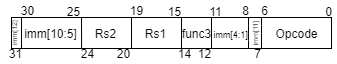
\includegraphics[width=0.7\textwidth]{sec1/images/Btype.png}
  \end{figure}
	\begin{description}
		\item Operands:\\
		\texttt{Rs1, Rs2, Immed-12}
		\item Instruction:\\
		\textsf{beq x4, x6, loop}\ \ \ \ $\longrightarrow$ \ \ \ \ \texttt{if x4 < x6, goto offset(pc)}
	\end{description}
	\item \textbf{U-type:}
  \begin{figure}[h]
    \center
    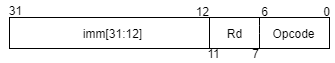
\includegraphics[width=0.7\textwidth]{sec1/images/Utype.png}
  \end{figure}
	\begin{description}
		\item Operands:\\
		\texttt{Rd, Immed-20}
		\item Instructions:\\
		\textsf{LUI x4, 0x12AB7}\ \ \ \ $\longrightarrow$ \ \ \ \ \texttt{x4 = value << 12}\\
		\textsf{AUIPC x4, 0x12AB7}\ \ \ \ $\longrightarrow$ \ \ \ \ \texttt{x4 = (value << 12) + pc}
	\end{description}
	\item \textbf{J-type:}
  \begin{figure}[h!]
    \center
    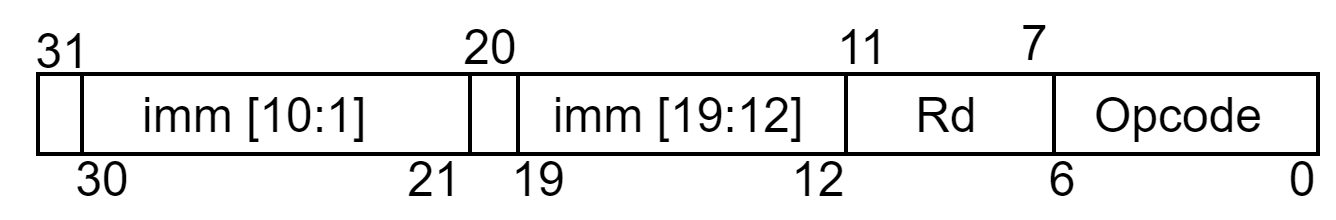
\includegraphics[width=0.7\textwidth]{sec1/images/Jtype.png}
  \end{figure}
	\begin{description}
		\item Instructions:\\
		\texttt{Rd, Immed-20}
		\item Example:\\
		\textsf{jal x4, func}\ \ \ \ $\longrightarrow$ \ \ \ \ \texttt{pc = pc + offset; x4 = return address}
	\end{description}
\end{description}
When the operation makes use of the immediate extracted directly from the instruction, sign extension is generally performed.\\ \\
The operations implemented in the lite version of the processor are:
\begin{description}
	\item Arithmetic:
	\texttt{add, addi, auipc, lui}
	\item Branches:
	\texttt{beq}
	\item Loads:
	\texttt{lw}
	\item Shift:
	\texttt{srai}
	\item Logical:
	\texttt{andi, xor}
	\item Compare:
	\texttt{slt}
	\item Jump and Link:
	\texttt{jal}
	\item Stores:
	\texttt{sw}
\end{description}
